\chapter{激励工具}
上一章我们批驳了一系列“貌似有理”的不写作的理由,传递的信息是清楚的:根据计划来安排写作。计划表造就了高效的写作者,这是他们为什么能写出那么多作品的原因。不过有可能你在计划的写作时间里无所事事:你坐下来,泡上咖啡,打开电脑,却不知道要写点什么。改过自新的突击写作者通常都不懂如何管理他们的写作时间。因为他们以往的激励工具是“最后期限”和“罪恶感”,他们没有规划目标、同时管理多个写作任务和执行计划的经验。本章将介绍一些常见的能够提升你的写作动机和提高写作成效的激励工具。这些工具起作用的前提是你已经在按照计划表行事。如果你还没有这样做,那你尽可以固执地继续你临时突击的节奏。

\section{制定目标}
和商人一样,学者也喜欢讨论目标。有些学者非常痴迷于目标、举措和战略计划,所以他们成了院长或教务长。目标值得我们好好关注。清晰的目标本身就是直接的激励——它们能够帮助人们制订计划,采取有效行动并因为目标达成而感到自豪(Bandura, 1997)。没有清晰的计划,人们的行动是散漫而毫无方向的(Lewin, 1935)。为了能够写得更多,你需要明确写作目标。这个并不像听上去那样容易,计划常常因为目标设定不当而跑偏方向。设定正确的目标可帮助你成为一个高效的写作者。

那么你该怎样设定目标呢?首先要意识到目标设定是写作过程的一个环节。花上一个写作时间段来好好理清你的写作目标是个不错的主意,我通常一个月整理一次。计划是写作的一部分,所以计划多的人写得也多。第二步是把你的目标逐条列出来——这些目标是具体的需要完成的写作任务。例如修改和重新提交论文,开始写一篇新的文章,接受邀请为某一本合集写一个章节,把你去年写了一半的那篇论文重新捡起来,写一篇课题经费申请报告,或是写一本书。

你想写些什么?当悔过的突击写作者首次设定目标时,通常只有一个任务——是过去三个月以来他们心头一直在回避的那个恐怖的任务。当然要把这个列出来,但是不能仅此而已。在未来的几个月里,你还有什么其他想写的呢?是否在看得见的将来就有一个课题申请要截止了?在你的文件柜里是否有一个还没有发表的实验数据值得你再好好琢磨一下?是否有一篇一直想写而未写的评论文章?把这本书暂时放下,找些纸来,天马行空地列一些你想写的东西。

你决定了要写些什么以后——也许这张单子看起来很长——现在你需要把这些目标写下来。在你的写作过程中不断更新这份东西是浪费时间,所以找一块白板或者公告板,放在你的写字台旁边,然后骄傲地把你的目标一一列在上面。一个突击写作者在这么长的计划面前会感到非常焦虑,但是你有时间表啊!你会自问 “我能完成吗?”自律性强的写作者会大致想一想要花几个星期来完成单子上列的这些内容。在这个单子上划去一项任务是非常令人开心的。你可以贴个笑脸在上面,如果这是你的风格的话。

第三步是把每天要写的目标尽可能具体化。当你真的坐下来为了你的目标奋斗的时候,你需要把这些目标变成一个个小的目标。 “修改这篇论文”是一个写作任务,但是对于决定要写些什么而言,这个表述过于宽泛了。每当你开始工作的时候,都需要花一点时间想一下当天你想完成些什么。“写论文”这样的目标太宽泛了,你需要具体的目标。这里列举一些具体目标的范例:
\begin{itemize}
  \item 至少写200个字;
  \item 把昨天写的草稿打印出来,阅读和修改;
  \item 制订新的写作目标并把它们写在白板上;
  \item 把总论部分的前三段写好;
  \item 补充所有参考文献,然后把引文和参考文献梳理清楚;
  \item 重读津泽(Zinsser, 2001)的书的第二十二章和第二十四章,给自己充充电;
  \item 继续把昨天的“设定目标”部分写完;
  \item 头脑风暴,然后把新论文的大纲写好;
  \item 重读评审人的评论并把要修改的部分一一列出;
  \item 校对清样并寄出。
\end{itemize}

有些人对在目标里列出字数和段落数感到很吃惊。记住,这些是具体的目标。要着手完成一个宽泛的目如——如“修改和重新提交这篇论文”——是很难的,但是要理解“至少写200个字”很容易——你坐下来,打字。精力旺盛的安东尼·特罗洛普(Anthony Trollope)写作的时候会戴一块手表,他的具体目标是15分钟写250个字(Trollope, 1883/1999)。一定要养成制订具体、集中、详细的写作目标的习惯,这样能够避免不知道做什么和不知道怎么做。


\section{挑选优先项}
现在,你手里有一张写作任务的清单了 。在所有这些任务里,你应该先做什么呢?我问了身边的写作高手们是怎样挑选优先项的。下面是综合我自己和身边高手的经验后给出的一些参考意见。你可以以此为参考,并挑选自己的优先项,把它们写在你的写作任务清单旁边。

{\kaishu 1.校对清样和复审论文}

这一项几乎是所有人的首选。道理很简单,校对清样是论文发表前的最后一步了,而且与其他很多学术写作任务不同,这一项通常有严格的时间节点。出版商们往往需要你快速地校对和复审,通常在48小时内完成。在经历了数月或数年的数据收集和写作过程之后.你为什么还会拖延自己的论文发表呢?快快完成吧。

{\kaishu 2.完成有截止期限的任务}

大多数的写作任务都没有截止期限,所以那些有截止期限的任务都应该在计划表中占有优先位置。有截止期限的任务可能包括受邀写作的部分章节、课题申请报告或是行政报告。有些期限很死——大多数的经费提供机构都过期不候,而有一些期限则比较灵活。就我个人而言,我并不把这一项列为我的优先选项,原因是我已经不像过去那样死抠截止期限了。如果你很好地执行了写作计划,那么你总是能够提前完成。截止期限对突击写作者来说是最大的激励,对于一个严格自律、有良好计划的写作者来说则没有什么用。

{\kaishu 3.修改论文以重新提交}

大多数的论文都会被拒。如果你有幸收到修改并重新提交的通知,千万别浪费了。重新修改后的论文比新提交的论文发表的几率高,所以你应把这一项列为优先项。

{\kaishu 4.评审稿件或课题申请报告}

这一项颇受争议。我的同事们就审稿是否应该被列为优先项有不同的意见。有些人认为这一项属于优先“非写作”项,应该快速完成,但不是用写作时间去完成。有些人对评审论文不怎么感冒,常常放在一边。不过我个人觉得这是一项颇为重要的工作,把它放在比较重要的位置。同行评审的过程与评审人关系甚大。心理学界的审稿流程之慢,已经影响到这个领域的发展。如果每个人都看得快一些,那么每个人也会写得欢快一些。快速地完成评论也有助于和编辑们建立良好的关系,因为他们总是对速度过慢的审稿人意见颇多。对于课题申请报告也是一样:课题评审对申请者而言事关重大,所以还是早点把它们做完为好。

{\kaishu 5.开始写作新的论文}

每一篇发表的论文都是从一份草稿起步的。从头写一篇新的论文对于突击写作者来说很难:他们常常花了几个月才开头,他们也是心血来潮时才做文献综述和数据分析部分的。其实,如果你能照着计划来,写一篇新的文章是相对容易的(与撰写课题申请报告、著作和修改论文相比)。第六章将就实证研究型论文写作给出一些建议。

{\kaishu 6.写各种杂文}

对所有不太重要但是仍然需要完成的写作任务,我们姑且称之为杂文。例如写一篇通讯短文。这能够帮助你暂时从那些主要的写作任务中解脱出来,捣鼓捣鼓些小玩意,获得片刻的安宁和乐趣。

几乎所有我调查的对象都提到,他们会把有研究生参与的写作任务放在特别优先的位置。比如,他们通常会花时间修改一篇要重新提交的论文,但是,如果要写一篇新论文,而这篇论文是与某个研究生合著的,他们会把它放在更为优先的位置。这是明智的建议。我也常常把优先权给那些我不参与实际写作的合著论文。试想一下,你辛辛苦苦地写了草稿,发给第二和第三作者征求修改意见,但是从来得不到反馈,这会是什么感觉?被合著者拖累是令人抓狂的,尤其是当这个合著者还不负责具体写作的时候。突击写作不是一个好习惯,而与人合著时还拖延则更加糟糕。

研究生应该和教授们有着不同的写作优先项。以下清单是我在采访了一些优秀研究生或是刚刚毕业的学生后整理的。

{\kaishu 1.有截止期限的写作任务}

研究生学习期间会有很多有截止期限的写作任务,例如某门课程的作业。很多学生抱怨他们的课程作业占用了太多写作时间,使得他们无法花更多的时间完成更为重要的写作任务,例如硕士论文。这是事实,但是截止期限就是截止期限,而这些小的作业或论文对未来的学术生涯未尝不是一种有益的尝试。如果你需要更多的时间写作,那只能在你的写作计划表里安排更长的时间。经费申请报告——例如研究生奖学金的申请——也同样有截止期限,而且它们非常重要,应该努力尽快完成。

{\kaishu 2.与学位授予相关的写作任务}

研究生学习期间,你需要写很多与学位授予相关的文章,例如硕士学位论文、综合考核报告、资格论文和博士学位论文。这些要想毕业就必须完成的东西最好快点写完。上述这些任务的成果有时候还能转化为可发表的论文,所以很多学生都会把与学位授予相关的论文与真正的专业写作结合起来。

{\kaishu 3.公开发表的专业论文}

科学研究只有在它公开发表,使之得以为同行所阅读和评论之后才能实现其真正的价值。你完成了论文,院系委员会也觉得你干得不错,但这是不够的,只有论文公开发表后学术界的其他同仁才能有机会更仔细地研究你的论文并认识它的价值。优秀的硕士学位论文或博士学位论文应该寄给专业的期刊。此外,你还应该力求在硕士学位论文和博士学位论文以外发表更多的专业论文。你要抓住每一个机会参与研究和专业写作。如果你很好地对写作加以规划,你将是你们项目里最高产的研究生。

{\kaishu 4.其他}

研究生常常写许多五花八门的文章,比如书评或报刊杂文。和其他类型的写作一样,写这一类的文章也是很好的锻炼,也很有意义。不过与专业水准的、存档留案的论文(比如期刊论文或专著的某个章节)比起来,这些杂文就显得不那么重要了。如果要在两个中间作出选择,那就应该把专业写作放在前面。

当我们在讨论选择优先项的时候,总有人会问:“那万一我觉得没什么可写呢?”对教授们来说,极少会感到没东西可写。恰恰相反,大多数我认识的教授都有堆积如山的未发表的数据。收集数据的过程是简单的,写作是困难的。如果你有一些十年前就已完成的实验却从未发表过,那我肯定你需要一段时间才会感到没有东西可写。更何况,写作促进写作。正如博伊斯(Boice, 1990)所发现的,那些定期写作的人会比那些只在灵感来临时写作的人有更多的创见(参见第二章)如果你觉得没有东西可写,那还是花一段写作时间来重新列一下你的写作目标吧。

然而,研究生们或许的确会觉得没有一个现在要跟进的写作任务。也许你刚刚完成了你的论文,暂时没有其他任务;也许你刚刚入学不久。别害怕,这个时候你有两个选择。首先,你可以参与一项正在进行的写作任务。你的导师,跟其他大多数的教授一样,或许正在为一大堆写作任务而头疼。敲开他/她的办公室然后说:“我最近看了一些关于如何成为更好的写作者的书,其中一本建议我敲开您的办公室,然后问问我是否能参与到一些写作任务中来。如果您有一些论文要写或是有一些数据要整理,我愿意帮忙。”很有可能你的导师会大倒苦水。教授们都希望自己的研究生在专业研究和写作方面倍加勤奋,所以你的导师一定会为你想加入而感到高兴。

另一个解决没有东西可写的办法是,你可以用写作时间来做些对专业发展有益的事。我读研究生时得到的最好的建议就是,“总是让自己不断思考”。研究生院是疯狂的,当你在为一大堆截止期限埋头奋斗的时候,你往往会忘了自己的长期目标。每周给自己留些固定时间,就能够利用它们来读些关于写作和教学的书,回顾自己的研究,想想你的职业规划。


\section{监控进展}
大多数人都不清楚自己究竟写了多少东西,是多是少。因为他们总是带着某种沾沾自喜、自我安慰的态度来审视自己,大多数人都认为自己比实际上要来得高效。为了写得更多,你必须带着某种冷峻、客观的态度来监控你的写作进展。有关自我管理的研究表明,仅仅设定目标和选定优先项是不够的:人们必须就达到目标的进程进行监控(Carver \& Scheier, 1998; Duval \& Silvia, 2001)。

监控写作进展有很多激励作用。首先,时时直面你的目标能够加深印象,防止你淡忘。许多人对如何管理他们写的东西很不在行。监控进展能够帮助你关注你正在进行的任务。其次,监控本身也足以帮助你坐下来开始写作。行为研究表明,自我观察本身就能够促进期待行为的发生(Korotitsch \& Nelson-Gray, 1999)。例如,想要存钱的人应该记录他们每天的花销,因为记录他们每天花了多少钱能够让他们节省开支。同理,想要定期写作的人应该追踪他们是否定期坐下来写作了:你放弃了某段写作时间,所以不得不在一个Excel表格里打上一个大大的“零”的时候,你会很奇怪地感到某种鞭策。最后,监控你的写作能够帮助你制订更合理的目标。经过一段时间,你将能积累足够的资料来合理地判断你大概需要多久来完成某项写作任务。制订更合理的目标,反过来又能够保障更高效的写作。

高产的写作者通常都会做这样或那样的监控。方法有很多种。在这部分里,我想介绍一下我的方法。每次我向别人介绍我的方法的时候,他们都给我一个诧异的表情,就好像听说我要拿伯尔尼山犬的毛来做被子似的。我用的系统看起来又蠢笨又牵强,还有点奇怪,不过它的确能帮助我集中精力。我有一个文件名是“写作进程.sav”的SPSS文件,图3.1是它的截图。我记录月份、日期、星期和年份。这些变量帮助我定位某一个日期。统计项是字数、目标和任务。在字数一栏,我键入每天我写的字数。字数统计工具能够轻松地告诉我文章的字数;每天开始和结束写作的时候都统计一下就能清晰地显示出一天的成果。你会注意到字数这一栏有很多空白。我之前已经强调过了,写作包含很多任务,不仅仅是码字。有时候我读些论文,有时候我填写课题申请表,有时候我重读需要修改并重新提交的论文。这些日子的字数一栏就会是空白的。设置目标一栏的目的就是回顾我是否完成了当天的目标。我个人的目标很简单,坐下来做些有利于推进研究的事,所以我会把这个变量记为\{0=未完成,1=完成\}。图3.1所示的那段时间我干得不错;只有7月5日那天我未完成我的既定目标,其他日子我都完成了。任务一栏用来描述我当天的任务。如实记录任务能够让你更清楚地知道你要花多少时间来完成一项任务。有时候会觉得某个任务没完没了,但是有可能它比你记忆中的已经简化了而你没有发觉。

\begin{figure}[!htb]
\label{fig3-1}
\centering
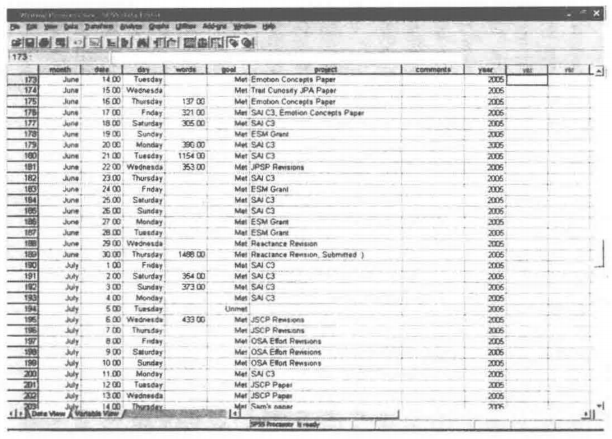
\includegraphics[width=0.9\textwidth]{fig3-1.png}
\caption{我用“写作进程.sav”文件来监控自己的写作进程}
\end{figure}

那些还死抱着各种无力借口的突击写作者可能会说“但是我不会用SPSS”或者“可是我只用SAS”!其实任何统计软件或者制表软件都可以做这件事,实在不行,画好线的笔记本和铅笔总是有的。监控本身才是关键,技术问题不是问题。不过,统计软件能够让你深入挖掘你的写作数据。如果你是一个统计控——这年头又有谁不是呢——那么你会爱上获得你的写作数据的感觉。我写了一个简单的SPSS公式来计算一些可见的数据和柱状图。当我开始写一篇新的文章时,我平均每天写789个字,如图3.2所示。听起来不是很多,不过字数逐日增加。图3.3显示的是每个月的目标完成情况。根据数据,在过去的12个月里,我在计划写作的日子中有97\%的日子实际坐下来写作了。我不是完美的,不过我对这个数据还是满意的。监控是为了改进,如果有一天这个数据达到100\%,我会感到非常骄傲。如果你很好奇,你还可以把目标达成情况和字数都按照天数来统计。所以,如果有人问我能写多少,我会回答97\%的工作日我都在写作,且每天我平均写789个字。他们可能会给我一个“伯尔尼山犬毛被子”的面孔,但这无所谓。

\begin{figure}[!htb]
\label{fig3-2}
\centering
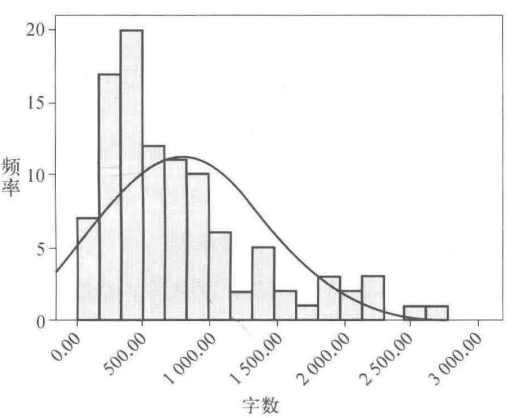
\includegraphics[width=0.9\textwidth]{fig3-2.png}
\caption{过去12个月每天的平均写作字数}
\end{figure}


\begin{figure}[!htb]
\label{fig3-3}
\centering
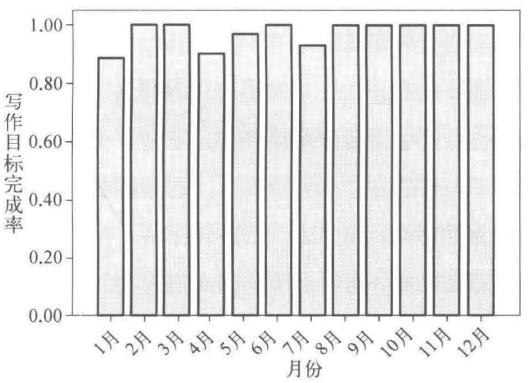
\includegraphics[width=0.9\textwidth]{fig3-3.png}
\caption{过去12个月每月的写作目标完成率}
\end{figure}


当你完成一项写作任务时,别忘了奖励自己。自我强化和依随性管理被证实对培养好习惯有很大的帮助(Skinner, 1987)。当你提交了一篇论文或是一份课题经费申请报告,给自己买杯好咖啡或是吃一顿奢侈的午餐,或者买一张古老的好莱坞-维克菲尔德式的书桌。写作的回报往往是滞后的——通常都要等上好几个月才能有杂志编辑或者经费评审委员会的消息——所以即时的自我奖励能够帮助你维持兴趣。不过,只有傻瓜才会以偷懒不写作的方式来奖励自己。永远不要以不写作的方式作为对写得好的奖励,以抛弃你的写作时间作为奖励,就好比以抽一支烟来奖励你戒烟成功。写作计划的有效执行有赖于超强的习惯掌控力:不要丢掉好的写作习惯。


\section{文思枯竭}
“等一下,”你也许会说,“到目前为止,这本书还没有提到任何关于文思枯竭的问题。当然啦,你可以制订计划,设定目标,然后监控进展,然而如果你实在写不出来怎么办?”我非常喜欢“文思枯竭”,这与我喜欢树精或是会说话的林中动物的道理是一样的——它们都很令人着迷,而且它们都不存在。当人们跟我说他们有时候真的会文思枯竭,我总是问他们,“你们到底要写什么?”学术写作者是不可能文思枯竭的。千万不要把自己和那些在艺术系教创作的朋友混为一谈。你又不是在创作一个长篇故事或是在写一个直指内心深处某个神秘角落的深刻隐喻。你对方差的精妙分析不会让读者们感动落泪,倒是有可能枯燥得让人掉眼泪。人们也不会影印你的参考文献目录并发给朋友们,期待能够给他们带去灵感与启迪。小说家和诗人是充满诗情画意的风景画家和肖像画家;学术写作者则是手握大型喷漆器重新粉刷地下室的油漆工。

文思枯竭是一个典型的倾向性谬论:对行为的描述同时被用来解释被描述的行为本身。所谓文思枯竭,说白了就是什么都没写。你说自己文思枯竭了,所以写不出东西,就相当于你说自己写不出东西是因为你什么都没写。这样的说法毫无意义可言。治疗文思枯竭的办法——如果你可以治愈无病呻吟——就是写作本身。建议重读第二章博伊斯(Boice, 1990)的实验。那个研究表明,苦苦挣扎的写作者们只要按照计划不断写作,就能写出很多东西——就这么简单。相反,那些非要等待“灵感”的人几乎什么也写不出。如果你真的文思枯竭,你有三个选择:(1)放下你手上正在摆弄的诗集,重新回到你的期刊论文写作中;(2)说服树精或会说话的动物们帮你写问题讨论部分;(3)重新制订你的写作计划,然后重新执行它。

就好像外星人只绑架相信存在外星人绑架事件的人一样,文思枯竭只会发生在相信有文思枯竭这回事的人身上。写作计划——这是个很神奇的东西——最神秘的部分就是,有计划的作者不会感到文思枯竭,不管到底有没有这回事。高效的写作者无论想不想写,都会按时写作。有时候他们写得不多——写作是件艰难的事情,但是不管怎样,他们都会坐下来写,不为那些虚无缥缈的事情所干扰。

\section{小结}
本章介绍了一些能够帮助你成为一个更高产的写作者的激励措施。制订好写作计划表以后,你需要确定写作目标并把它们写下来。然后,在你坐下来写作以前,先花一分钟想一想你今天想干什么。选定优先项能够马上帮助你摆脱同时进行多个写作任务的压力。监控你的写作能够让你集中精力完成目标,监督你不要放弃任何一天,告诉你你能写得多好,还能提供足够的数据让那些怀疑你的突击写作者闭嘴。任何能把本章提到的建议都一一做到的人,毫无疑问都能写得很多。